\documentclass[12pt,twoside,notitlepage]{report}

\usepackage{a4}
\usepackage{verbatim}

\input{epsf}
\usepackage[pdftex]{graphicx}

\usepackage{listings}
\lstset{basicstyle=\footnotesize\ttfamily,breaklines=true}

\raggedbottom                           % try to avoid widows and orphans
\sloppy
\clubpenalty1000%
\widowpenalty1000%

\addtolength{\oddsidemargin}{6mm}       % adjust margins
\addtolength{\evensidemargin}{-8mm}

\renewcommand{\baselinestretch}{1.1}    % adjust line spacing to make
                                        % more readable

\setcounter{secnumdepth}{2}				% make all subsubsections appear in the table of contents
\setcounter{tocdepth}{5}

\begin{document}

\bibliographystyle{plain}


%%%%%%%%%%%%%%%%%%%%%%%%%%%%%%%%%%%%%%%%%%%%%%%%%%%%%%%%%%%%%%%%%%%%%%%%
% Title


\pagestyle{empty}

\hfill{\LARGE \bf David Barker}

\vspace*{60mm}
\begin{center}
\Huge
{\bf Functional Reactive Programming for Data Binding in C$\sharp$} \\
\vspace*{5mm}
Computer Science Tripos Part II \\
\vspace*{5mm}
Jesus College \\
\vspace*{5mm}
\today  % today's date
\end{center}

\cleardoublepage

%%%%%%%%%%%%%%%%%%%%%%%%%%%%%%%%%%%%%%%%%%%%%%%%%%%%%%%%%%%%%%%%%%%%%%%%%%%%%%
% Proforma, table of contents and list of figures

\setcounter{page}{1}
\pagenumbering{roman}
\pagestyle{plain}

\chapter*{Proforma}

{\large
\begin{tabular}{ll}
Name:               & \bf David Barker \\
College:            & \bf Jesus College \\
Project Title:      & \bf Functional Reactive Programming for \\
					& \bf Data Binding in C$\sharp$ \\
Examination:        & \bf Computer Science Tripos Part II \\
Word Count:         & \bf TBC \\
Project Originator: & Tomas Petricek \\
Supervisor:         & Tomas Petricek \\
\end{tabular}
}


\section*{Original Aims of the Project}

Aims of the project will go here.


\section*{Work Completed}

Work completed will go here.

\section*{Special Difficulties}

None
 
\newpage
\section*{Declaration}

I, David Barker of Jesus College, being a candidate for Part II of
the Computer Science Tripos, hereby declare that this dissertation
and the work described in it are my own work, unaided except as may
be specified below, and that the dissertation does not contain
material that has already been used to any substantial extent for a
comparable purpose.

\bigskip
\leftline{Signed [signature]}

\medskip
\leftline{Date [date]}

\cleardoublepage

\tableofcontents

\listoffigures

\newpage


%%%%%%%%%%%%%%%%%%%%%%%%%%%%%%%%%%%%%%%%%%%%%%%%%%%%%%%%%%%%%%%%%%%%%%%
% Chapters start here

\cleardoublepage

\setcounter{page}{1}
\pagenumbering{arabic}
\pagestyle{headings}


%%%%%%%%%%%%%%%%%%%%%%%%%%%%%%%%%%%%%%%%%%%%%%%%%%%%%%%%%%%%%%%%%%%%%%%
% Introduction

\chapter{Introduction}

It has become a firmly established practice when writing applications to separate the code managing the user interface from the business logic powering it. This is a key part of the principle of separation of concerns, and means that the interface can be safely changed without needing to modify the backend code (and vice versa, assuming the backend provides a consistent interface). Beginning with the traditional MVC architecture, this has led to the development of a family of system architectures such as MVPM and MVVM which enforce this principle.

\section{Data binding}

Data binding presents a mechanism for bridging the gap between the separated layers by allowing the developer to specify that some value in the user interface code should be bound to a property of the model. This usually simply means that whenever the value in the model changes, the data binding framework will ensure that the value in the user interface is also updated to the same value. However, bindings can often be more complex: for instance, there could be a text box in the user interface which reflects backend data but can also be used to change it (two-way binding). Alternatively, there might be a user interface component whose value is determined by some function of a variable in the model - consider a list view which displays a filtered and sorted version of a list stored in the model. There could even be values which depend on multiple sources, or more complex many-to-many bindings.

Many current languages and frameworks provide data binding features with varying levels of complexity. Java has a variety of extension libraries [examples] which allow the programmer to use data binding with Swing. Javascript too has a variety of possibilities, with a prominent example being the backbone.js MVC framework. Unfortunately, many of these are quite limited and difficult to use - backbone.js, for example, only provides one-way binding and requires a lot of boilerplate code from the programmer.

\section{Data binding in .NET}

Microsoft’s .NET framework offers a particularly powerful example of data binding through Windows Presentation Foundation (WPF). Based on the MVVM architecture, it has many features to allow things like two-way binding, binding through functions and bindings based on list operations. One of its key advantages is that the user interface can be defined entirely in XAML \footnote{Extensible Application Markup Language, an XML-based markup language for defining user interfaces and simple behaviour} with bindings being specified through XAML parameters. The view logic is then specified in the ViewModel which in turn communicates with the model. This means user interface designers can work purely in XAML without concern for the logic or binding mechanisms in place behind the scenes.

However, WPF suffers from a similar problem to many other data binding frameworks: advanced data bindings can be very complex and difficult to manage, and setting up bindings in the first place requires quite a lot of boilerplate code in the model and view. Furthermore, binding through functions requires special ‘value converter’ classes to be written. This is essentially an application of the Template pattern, and the value converters are not type safe - they take objects as input and return objects as output (and bindings with multiple inputs will simply take arrays of objects with no guarantee that the right number of values has been passed). [Maybe more disadvantages?] Clearly a more simple and general binding framework would definitely make application development simpler.

\section{Project inspirations}

Many useful ideas for data binding come from the area of functional programming. Functional reactive programming (FRP), for example, is a paradigm which nicely models the concept of data binding in a general way. Another useful concept is that of the ‘arrows’ implemented in Haskell. An ‘arrow from type A to type B’ essentially represents a process taking an input of type A and returning something of type B, and these can be arbitrarily combined in interesting ways to build up complex functions. More detail on both will be given in the next chapter.

The FRP paradigm was the inspiration for the project, which sought to implement a general-purpose data binding framework in C$\sharp$ using concepts derived from functional programming. I successfully implemented a framework which provides data binding in both directions, through arbitrary functions with arbitrary numbers of inputs and outputs, all with a simple syntax based on lambda expressions. Minimal boilerplate code is required to set up bindable properties - the containing class should extend Bindable, and from there marking arbitrary member variables and properties with the [Bindable] tag will make it possible to create bindings to and from them with a single function call. I also implemented a large variety of arrow types and arrow operators along with a number of utility functions to make creating and combining them simple.

\cleardoublepage


%%%%%%%%%%%%%%%%%%%%%%%%%%%%%%%%%%%%%%%%%%%%%%%%%%%%%%%%%%%%%%%%%%%%%%%
% Preparation

\chapter{Preparation}

This chapter is empty still!

\cleardoublepage


%%%%%%%%%%%%%%%%%%%%%%%%%%%%%%%%%%%%%%%%%%%%%%%%%%%%%%%%%%%%%%%%%%%%%%%
% Implementation

\chapter{Implementation}

\section{Overview}

Give a general overview


\section{Arrows}

\subsection{Overview}

Overview of how arrows worked

\begin{itemize}
	\item Type inference chosen instead of reflection
	\item Techniques for allowing type inference - static constructor methods, extension methods etc.
	\item Arrow intercompatibility?
	\item Multiple inputs/outputs and the decision to use C$\sharp$ Tuple class
\end{itemize}

\subsection{Simple arrows}

Summarise functionality, combinators and syntactic efforts made here, mention things like the parallelism of the And operator as well.

\subsubsection*{Challenges encountered}

A few - mention type inference challenges, overcoming type system whilst maintaining type safety and difficulties with the And operator (also alternatives considered for this)

\subsection{Invertible arrows}

Discuss the alternative ways of implementing this - a set of preset arrows designed to form a Turing-complete basis, forcing the user to specify an arrow for each direction etc. Final decision to simply construct using a function for each direction then allow arbitrary combination, as inspired by the paper on invertible arrows.

\subsection{List arrows}

\begin{itemize}
	\item Wrapping Linq
	\item SQL-style syntax - helped by various extension methods
	\item Functional-style operations - foldl and foldr
\end{itemize}

\subsection{Choice arrows}

\begin{itemize}
	\item Not deeply implemented or tested but could be handy for some things, most likely convenient exception handling
	\item This wouldn't be much good for bindings though
\end{itemize}

\subsection{Further utility arrows}

\begin{description}
	\item[Identity arrows] Exist for normal arrows and invertible ones; mention the reason for the class - has to be type parameterised
	\item[Tuple reassociation arrows] Useful for stuff like arrow law tests, explain here...
	\item[Others] Any more to mention?
\end{description}

\subsection{Feedback in arrows}

Discuss whether this would be useful or not, reasons for it not being there (lack of real-world use cases?) and how one might implement it.


\section{Data binding}

\subsection{Overall architecture}

Use diagrams and stuff to explain it.

\subsection{Creating bindable sources and destinations}

One of the main problems with WPF data binding is the complexity of making sources 'bindable'. This usually requires that the programmer manually implement the \texttt{INotifyPropertyChanged} interface, creating appropriate events and overriding the set methods of all their properties such that they throw the right events. This often becomes a case of copying and pasting the code used for other data sources as it is almost always identical and includes boilerplate tasks like ensuring a variable's new value is different from its old one before throwing the event, and checking that the event isn't null.

For this project I decided to abstract these details away into a base class, called \texttt{Bindable}. This provides events for binding and a set of methods used by binding classes to manage data binding, many of which will be discussed later in this section. The most important are those which allow getting and setting of arbitrary variables by name using reflection, as these are the main interface used by the bindings manager. These have been designed to be dynamically type safe (that is, throwing exceptions at run time where type errors are encountered), to ensure the properties being accessed exist and to abstract away the differences between properties and simple public member variables\footnote{WPF does not allow binding to member variables, but for this project I decided there was no obvious need to distinguish between the two}.

The result of this is that instead of writing all the boilerplate code one would usually write, the programmer need only make their sources and destinations extend Bindable and all the usual things will be handled elsewhere leading to considerably less code clutter. A representative example of the final syntax is given in Listing \ref{lst:bindable_source_class}.

Another addition that can be seen in the listing is the \texttt{[Bindable]} attribute which has been used above the \texttt{value} property. This uses a PostSharp aspect, explained in the next section, to intercept the setter for throwing events and so relieve the programmer of having to do this themselves.

\begin{lstlisting}[language={[Sharp]C}, caption={Creating a bindable source class}, label=lst:bindable_source_class]
public class DataSource : Bindable
{
	[Bindable]
	public int value { get; set; }
}
\end{lstlisting}

\subsubsection*{PostSharp}

PostSharp is a C$\sharp$ extension which provides aspect-oriented programming (AOP) functionality. Essentially, AOP is a means of separating cross-cutting concerns from the code they affect, allowing 'aspects' to be written providing this common functionality. Markers can then be placed in the appropriate points, and the aspects will generate and inject their code into these locations at compile time.

In this case, the \texttt{Bindable} aspect will intercept the setter of any property or member variable it is placed above and insert code to check whether the value has changed and throw appropriate events if it has. This does not interfere with any setters the programmer may already have specified, as it defers to the programmer's setter before throwing the event for the value changing (thus ensuring the event is only thrown once all values are updated and any side-effects have occurred).

Unfortunately, the project budget only extended as far as the free version of PostSharp. Syntax for bindings could likely have been improved even further using the method and property introduction features provided by the full version, as this would have removed the need to extend Bindable. The unfortunate side-effect of the Bindable base class is that the class can no longer extend any other base class, as C$\sharp$ does not allow multiple class inheritance. However, in working with the binding framework it was found that this rarely caused problems that couldn't be worked around, and in any case patterns exist to overcome the lack of multiple inheritance in the general case\footnote{The 'composition over inheritance' pattern is one such technique which uses a shared base interface and a proxy object to 'inherit' from a class without inheriting}.

\subsection{Creating bindings}

It was decided that it would make sense to manage all bindings in a given project centrally, so that constraints on cycles and conflicts can be enforced and bindings can be dynamically added and removed. Therefore, the \texttt{BindingsManager} class was implemented to create and maintain bindings. This is a static class handling all bindings for the project it is used in and exposing methods for creating and removing particular bindings. The programmer can call it passing in the sources, destinations and arrow they wish to use, and it will return a binding handle which they can use to remove the binding later if needed. The bindings manager also handles cycle and conflict detection, automatic creation of two-way bindings based on the arrow type and support for many-to-many bindings, all of which will be explained in this section.

\subsubsection{Syntax and usage}

In order to abstract away details like types and specific object references, the bindings manager operates on 'bind points' -- essentially, structures containing a reference to the \texttt{Bindable} source and a string representation of the property or member variable being bound. An extension method was written to make creating these simpler, as calling the constructor with the object and variable name turned out to make the overall syntax fairly cluttered. The standard way of making a bind point for an object 'obj' with property 'value' is thus \texttt{obj.GetBindPoint("value")}, which is a lot simpler to write.

Basic bindings (that is, from one source to one destination in one direction) can be set up by passing in a source bind point, and arrow to use for the binding and a destination bind point. An example of this is given in Listing~\ref{lst:creating_simple_binding}.

\begin{lstlisting}[language={[Sharp]C}, caption={Creating a binding between two properties}, label=lst:creating_simple_binding]
BindingsManager.CreateBinding(
	source.GetBindPoint("value"),
	arrow,
	destination.GetBindPoint("result"));
\end{lstlisting}

\subsubsection{Cycle and conflict detection}

Techniques used and all that.

\subsubsection{Two-way binding}

Problems encountered - need for variable ‘locking’ system to avoid infinite loop

\subsubsection{Many-to-many bindings}

Many-to-many bindings presented an additional challenge for the binding system. It was decided that the best approach in terms of syntax would be to have the user pass in a list of source bind points, an arrow and a list of destination bind points, so as to mirror the syntax used in simple bindings. However, this simple approach is out of step with the way parameters are passed to arrows: by construction, all arrows taking multiple inputs will take them in the form of a binary-tree-structured Tuple\footnote{This can be verified by looking at the implementations of the operators; for instance, And converts two arrows (which may be on tuples) into an arrow on two-tuples containing the types of the original arrows, thus building up a binary tree structure}. As there didn't appear to be any C$\sharp$ syntax allowing the user to pass in binding sources in a similar fashion (such that the structure could be understood by the binding), it was decided that an argument marshaller/unmarshaller would be needed to handle the translation between lists of bind points and tree-structured tuples.

\begin{figure}[!ht]
  \centering
  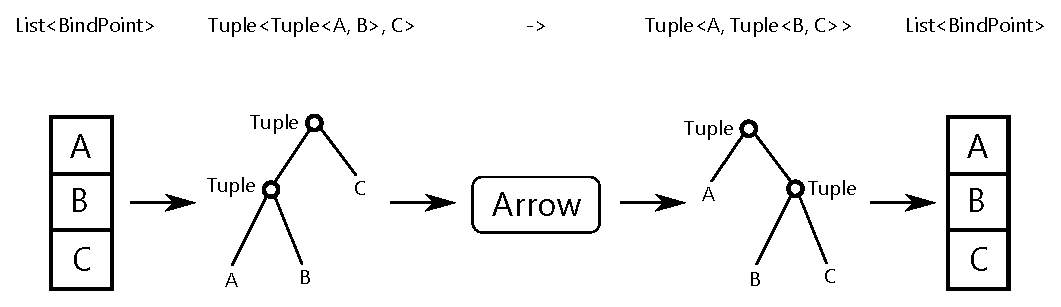
\includegraphics[width=\textwidth]{fig/ArgumentMarshalling.pdf}
  \caption{Marshalling a list of BindPoint sources to pass to an arrow and unmarshalling the result}
  \label{fig:argument_marshalling}
\end{figure}

By using reflection on the type of the arrow, I was able to convert a list of bind points to a binary-tree-structured Tuple. The code essentially does a recursive depth-first search through the input type of the arrow (obtained via reflection), simultaneously constructing a Tuple of the same structure and inserting values from the bind points wherever a 'leaf' is encountered in the type being searched. At the other end, a similar process is used to extract the values from the returned tuple and put them into a list which is then used to assign to the destination bind points. The process is illustrated in Figure~\ref{fig:argument_marshalling}, where a set of inputs of types A, B and C are being passed into an arrow from type \texttt{Tuple<Tuple<A, B>, C>} to type \texttt{Tuple<A, Tuple<B, C>>}.

\subsubsection{Problems encountered}

\paragraph{Type safety}

All sort of problems here; difficulties of type checking arrows should also be mentioned.

\paragraph{Binding to lists}

They don't throw events! Binding to lists needs the list to be ‘assigned’ to for it to update. Possible solutions like ObservableEnumerable (or whatever it was called), potentially more boilerplate, future work ‘n’ shit.

\subsection{Integration work with WPF}

Mention difficulties with the value converter and inability to properly integrate it into XAML and stuff.

\cleardoublepage


%%%%%%%%%%%%%%%%%%%%%%%%%%%%%%%%%%%%%%%%%%%%%%%%%%%%%%%%%%%%%%%%%%%%%%%
% Evaluation

\chapter{Evaluation}

\section{Correctness of arrow implementations}

Mention here that the main device for determining their correctness has been the arrow laws, and possibly list them with explanations? Also mention that 'special' arrows like ListArrows are correct because they are based on simple arrows and invertible arrows. Also, maybe say that ArrowChoice was ignored here as it's slightly extraneous and its correctness probably follows from the correctness of simple arrows anyway.

\subsection{Automated testing}

\subsubsection{Simple arrows}

Give tests and results for arrows.

\subsubsection{Invertible arrows}

Same for invertible arrows.

\subsection{Correctness proof by decomposing into lambda calculus}

Explain the technique used to translate into lambda calculus and the likely correctness of this, and give a few sample proofs for some non-trivial arrow laws.

\section{Syntax evaluation}

\subsection{Arrow syntax}

Arrow syntaxy stuff.

\subsubsection{Comparison with Haskell}

Might not be great, but why not?

\subsection{Binding syntax}

Pretty good. Say something about the demo apps and stuff:

\subsubsection{Username two-way binding}

Todo

\subsubsection{List binding from a mock database}

Todo

\subsubsection{Some other demo}

Todo

\section{Performance testing}

\subsection{Arrow performance}

Tests indicating how arrows perform vs. functions and funcs.

\subsubsection{Measuring technique}

Explain how the results were obtained

\subsubsection{Simple function results}

The simple function results can be seen in the graph.

\begin{figure}[!ht]
  \centering
  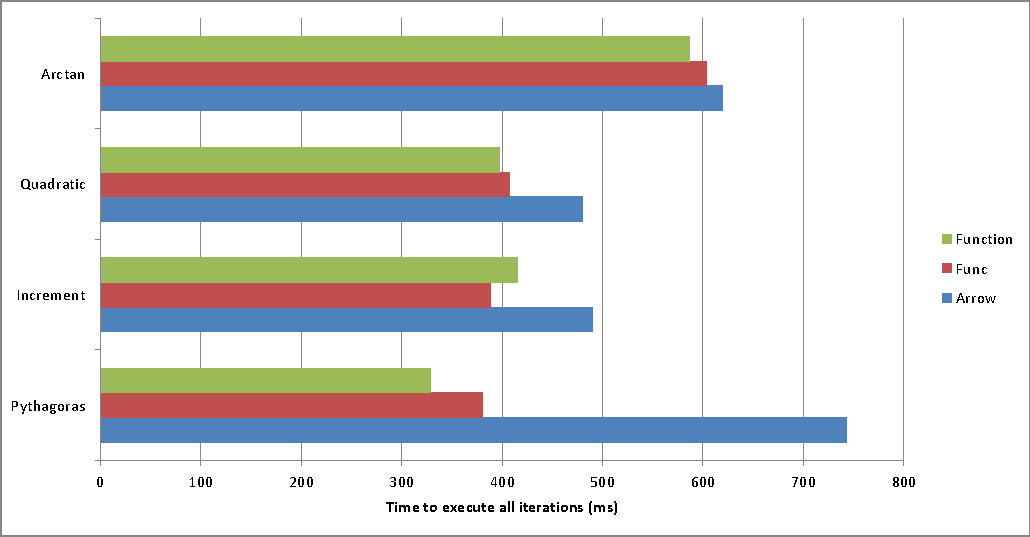
\includegraphics[width=\textwidth]{fig/SimpleFunctionPerformanceChart.pdf}
  \caption{Performance of arrows, Funcs and normal functions in implementing simple functionality}
  \label{fig:simple_function_performance}
\end{figure}

\subsubsection{List function results}

Results for list-based functions

\begin{figure}[!ht]
  \centering
  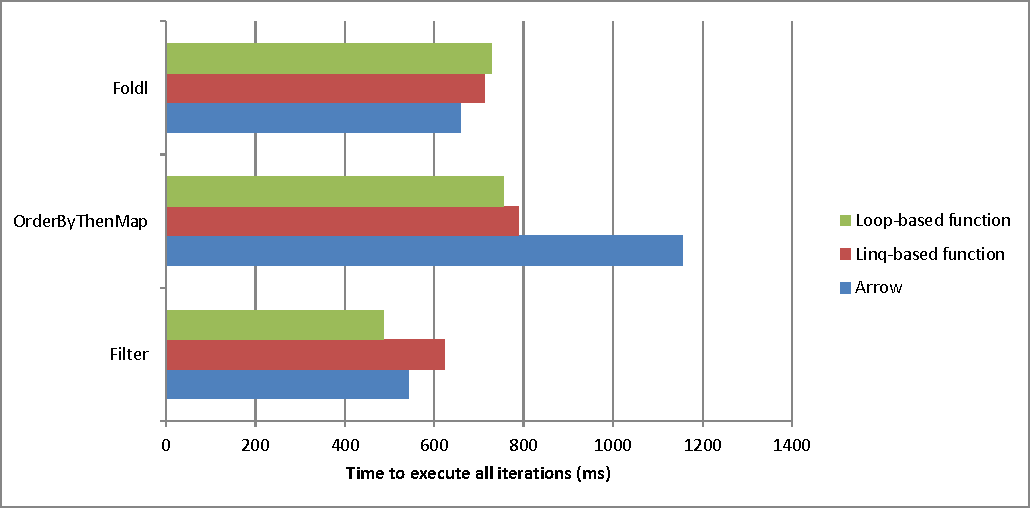
\includegraphics[width=\textwidth]{fig/ListFunctionPerformanceChart.pdf}
  \caption{Performance of arrows, Linq queries and normal (loop-based) functions in implementing simple list functionality}
  \label{fig:list_function_performance}
\end{figure}

\subsubsection{Overhead due to arrow chaining}

Explanation of the problem (which will have been highlighted in earlier results) along with test results for increasingly long chains of identity functions. Suggest reasons for this and potential solutions (or maybe the solutions should come in later?)

\subsection{Binding performance}

Todo...

\cleardoublepage


%%%%%%%%%%%%%%%%%%%%%%%%%%%%%%%%%%%%%%%%%%%%%%%%%%%%%%%%%%%%%%%%%%%%%%%
% Conclusion

\chapter{Conclusion}

Conclusion goes here!

\cleardoublepage


\end{document}